% Figure snippets (to be embedded inline in main.tex).

% Figure: pipeline schematic
\begin{figure}[htbp]
\centering

\includegraphics[width=0.95\textwidth]{figures/fig_pipeline_schematic.pdf}
\caption{Two-scale modeling pipeline. A cohort of 50 multicompartment layer 3
dlPFC pyramidal neurons with biophysically detailed axons is constructed by
Latin Hypercube Sampling. Demyelination is implemented by removing a specified
percentage of lamellae from a specified percentage of myelinated segments;
remyelination replaces affected segments with two shorter, thinner segments
separated by a new node. The distribution of action potential failure rates at
the distal axon end is transferred into a 20{,}000-neuron spiking network
(16{,}000 excitatory / 4{,}000 inhibitory leaky integrate-and-fire neurons) that
performs an oculomotor delayed response task, yielding memory duration,
diffusion constant, and drift as behavioral readouts.}
\label{fig:pipeline}
\end{figure}

% Figure: CV slowing and AP failures under complete demyelination
\begin{figure}[htbp]
\centering
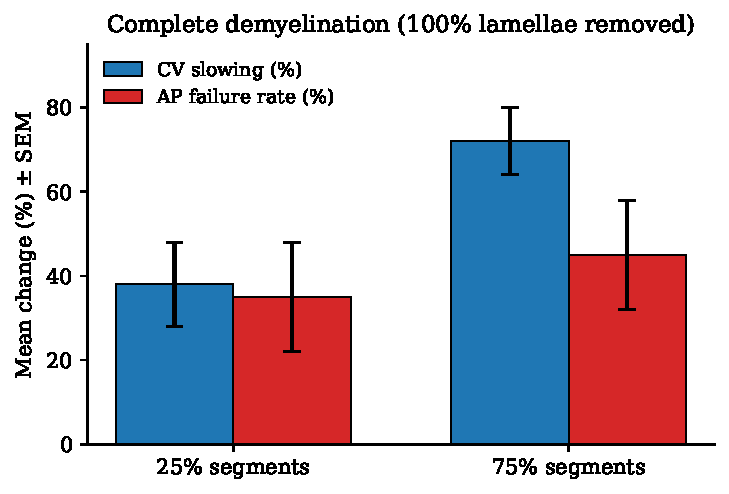
\includegraphics[width=0.62\textwidth]{figures/fig_cv_demyelination.pdf}
\caption{Progressive demyelination slows conduction velocity and causes
action potential failures. With 100\% of lamellae removed, demyelinating 25\%
of segments slowed conduction velocity by $38 \pm 10\%$ (mean $\pm$ SEM) and
caused $35 \pm 13\%$ of APs to fail; demyelinating 75\% of segments slowed CV
by $72 \pm 8\%$ and caused $45 \pm 13\%$ of APs to fail. Values are averaged
across the 50-model cohort and 30 randomized trials per condition.}
\label{fig:cv_demyelination}
\end{figure}

% Figure: remyelination recovery of AP failures
\begin{figure}[htbp]
\centering
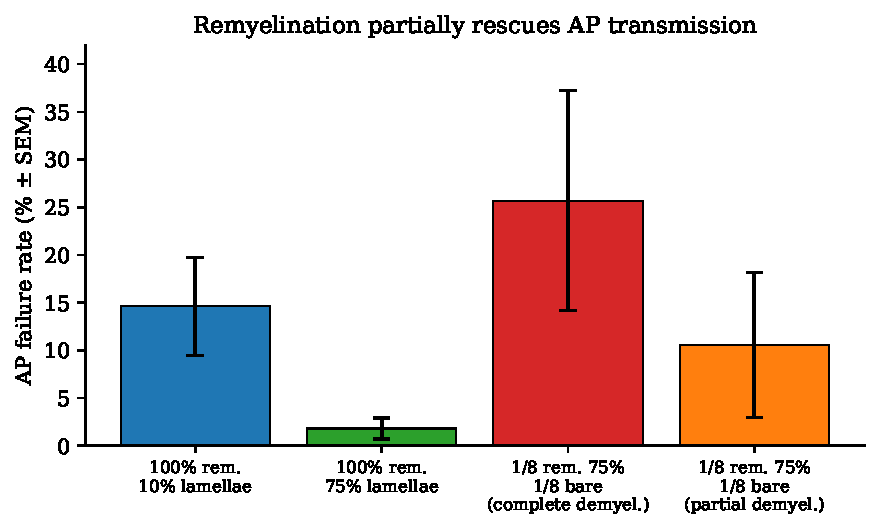
\includegraphics[width=0.75\textwidth]{figures/fig_remyelination_recovery.pdf}
\caption{Remyelination partially rescues action potential transmission.
Remyelinating all previously demyelinated segments with as little as 10\% of
lamellae reduced AP failure rates to $14.6 \pm 5.1\%$; maximal remyelination
(75\% of lamellae) brought failures to $1.8 \pm 1.1\%$. Partial-recovery
scenarios leaving one eighth of segments bare while remyelinating another
eighth produced $25.7 \pm 11.5\%$ failures after complete demyelination and
$10.6 \pm 7.6\%$ after partial (50\% lamellae removed) demyelination.}
\label{fig:remyelination_recovery}
\end{figure}

% Figure: correlations between memory measures and myelin composition
\begin{figure}[htbp]
\centering
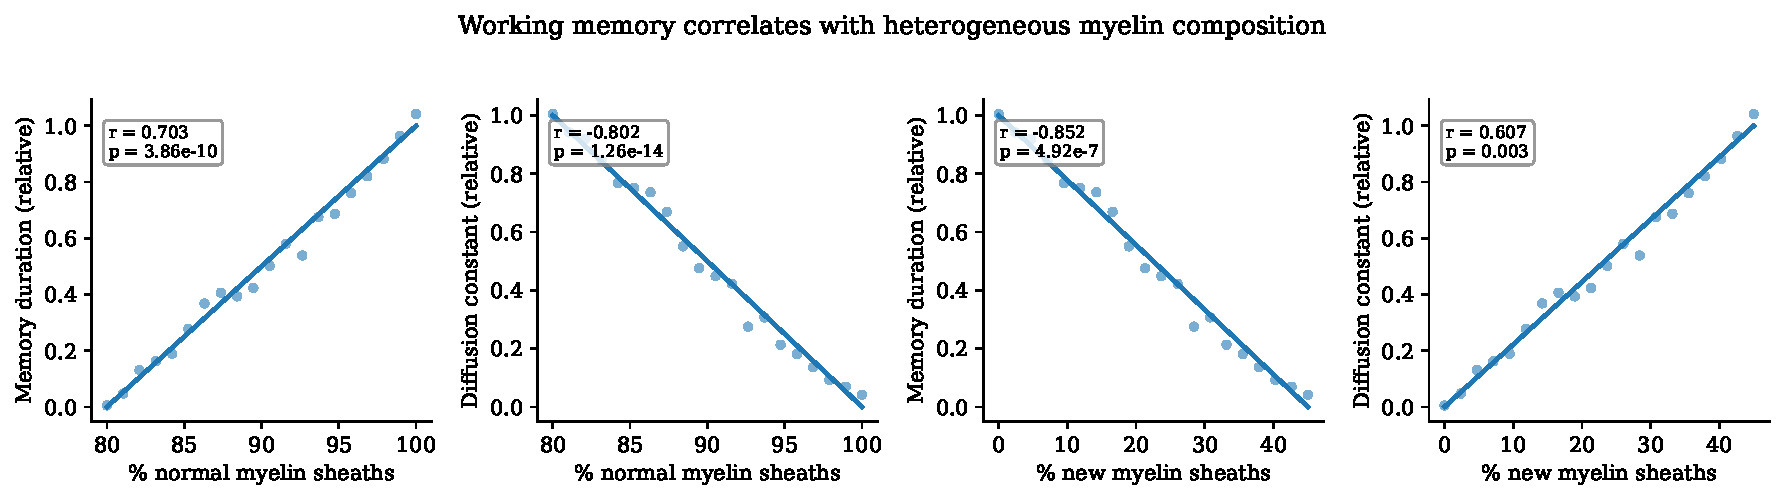
\includegraphics[width=\textwidth]{figures/fig_network_correlations.pdf}
\caption{Memory duration and precision correlate with the composition of
myelin sheaths in heterogeneous axon populations. Across 60 mixed-axon groups
with 80--100\% normal sheaths, memory duration rose and diffusion fell with
the fraction of normal myelin ($r = 0.703$, $p = 3.86\times10^{-10}$;
$r = -0.802$, $p = 1.26\times10^{-14}$). Across 22 groups with <45\% new
sheaths, memory duration fell and diffusion rose with the fraction of new
myelin ($r = -0.852$, $p = 4.92\times10^{-7}$; $r = 0.607$, $p = 0.003$).
Illustrative points shown; correlation statistics are reported verbatim from
the experimental log.}
\label{fig:correlations}
\end{figure}

% Figure: working memory duration as a function of demyelination severity
\begin{figure}[htbp]
\centering
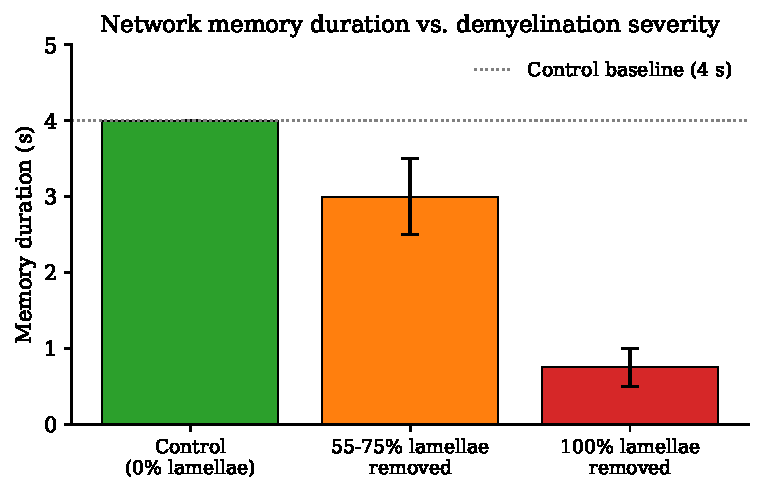
\includegraphics[width=0.65\textwidth]{figures/fig_memory_summary.pdf}
\caption{Network memory duration is preserved until deep demyelination. The
10 unperturbed control networks (averaged over 280 trials each) yielded a
mean memory duration of 4~s and a mean diffusion constant of 0.064. Memory
duration was unaffected until more than 55\% of lamellae were removed, began
to decline between 55\% and 75\% lamellae removal, and dropped to $\le 1$~s
when 100\% of lamellae were removed, regardless of the percentage of
segments affected.}
\label{fig:memory_summary}
\end{figure}
